
Raspbian ist das offizielle Betriebssystem f�r den Raspberry~Pi. F�r die Verwendung bei einem Raspberry Pi Jam wurde die Distribution \texttt{Raspjamming} vom Grazer Computer Club (GC2) erstellt. Ausgehend vom Raspbian Lite Image wurde noch verschiedene Entwickerlerprogramme und Werkzeuge installiert. Zus�tzlich wurde das System so eingerichtet, dass der Raspberry Pi Zero direkt �ber den USB-OTG Anschluss mit dem Host-PC verbunden werden kann. Der SSH-Dienst und WLAN wurde aktiviert. Alle L�ndereinstellung wurden von UK auf �sterreich/German ge�ndert. Ein Web-Server stellt Programme und Hilfe zur Verf�gung. Somit ist ein Betrieb auch ohne Internetverbindung m�glich. Ein Download-Link zum aktuellen Raspjamming-Image wird auf der GitHub Projekt-Seite \urlsmall{https://github.com/GrazerComputerClub/Raspjamming-Image} zur Verf�gung gestellt.\\  
F�r die Installation ben�tigt man eine mindestens 4~GB gro�e MicroSD-Karte und einen Computer mit MicroSD-Kartenleseger�t (USB-Adapter oder Karten-Slot mit Adapter).


\subsection{Linux - Etcher}

Nach dem Download von \urlsmall{https://github.com/GrazerComputerClub/Raspjamming-Image/releases} liegt das Image als komprimierte ZIP-Datei vor.\\ 
Das grafische Programm Etcher (Download auf \url{https://www.balena.io/etcher/}) kann direkt zum �bertragen der komprimierten Image-Datei verwendet werden. 

\begin{console}
	wget https://github.com/balena-io/etcher/releases/download/v1.5.43/\
	balena-etcher-electron-1.5.43-linux-x64.zip
	unzip balena-etcher-electron-1.5.43-linux-x64.zip
	sudo mv balenaEtcher-1.5.43-x64.AppImage /usr/local/bin/etcher
	etcher &
\end{console}


%Nach dem Starten wird danach gefragt ob eine Verkn�pfung zum Programm erstellt werden soll. Dies sollte man mit "`Yes"' beantworten.\\ 
Mit der Schaltfl�che "`Select image"' kann man die Zip-Datei "`20\_\_-\_\_-\_\_-Raspjamming-full.img.zip"' ausw�hlen. Ist nur ein m�gliches Ziel vorhanden, wird es bereits vorausgew�hlt, z.~B. die MicroSD-Karte im Karten-Slot (/dev/memcblk0) oder im USB-Adapter (/dev/sdb). Sind mehrere m�gliche Ziele vorhanden, wird die "`Select drive"' Schaltfl�che freigeschaltet. Dann kann ein Laufwerk manuell ausgew�hlt werden.

\begin{figure}[ht]
	\centering
	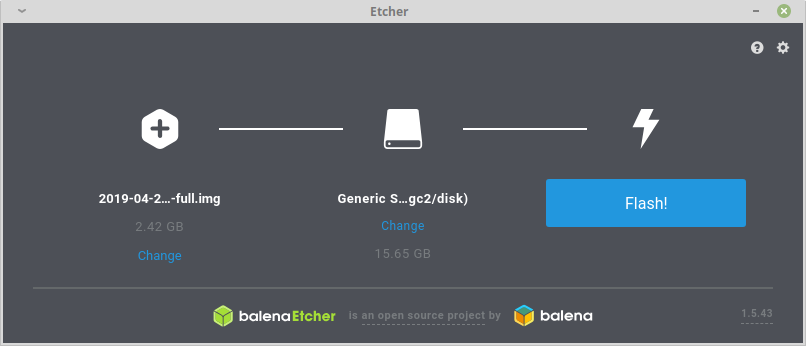
\includegraphics[scale=0.3]{images/Etcher.png}
	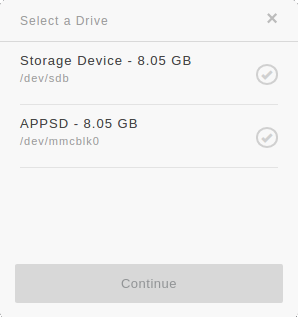
\includegraphics[scale=0.3]{images/Etcher_2.png}
	\label{Etcher}
\end{figure}


Wenn man noch etwas �ndern will, kann die entsprechende "`Change"' Schaltfl�che ausgew�hlt werden. Zum Schluss wird der Schreibvorgang mit der "`Flash!"' Schaltfl�che gestartet. M�glicherweise wird vom Programm allerdings noch das System-Passwort abgefragt.\\ 
Das Laufwerk bzw. die Partitionen werden nun aus dem System ausgeh�ngt und der Schreibvorgang gestartet. Der Fortschritt, die durchschnittliche �bertragungsrate und die Restlaufzeit werden w�hrend des Vorgangs angezeigt.


\subsection{Windows - Rufus}

Nach dem Download von \urlsmall{https://github.com/GrazerComputerClub/Raspjamming-Image/releases} liegt das Image als komprimierte ZIP-Datei vor. Es kann mit dem Programm "`Rufus"' (Download auf \url{https://rufus.akeo.ie/}) direkt auf eine MicroSD-Karte �bertragen werden. Dazu klickt man auf "`AUSWAHL"' und w�hlt dann die Zip-Datei "`20\_\_-\_\_-\_\_-Raspjamming-full.img.zip"' aus. Unter Laufwerk w�hlt man das Laufwerk aus, in dem sich die zu schreibende MicroSD-Karte befindet. Achtung: Die Daten von dem Laufwerk werden �berschrieben! Nach dem Dr�cken von "`Start"' beginnt der Schreibvorgang.

\begin{figure}[ht]
	\centering
	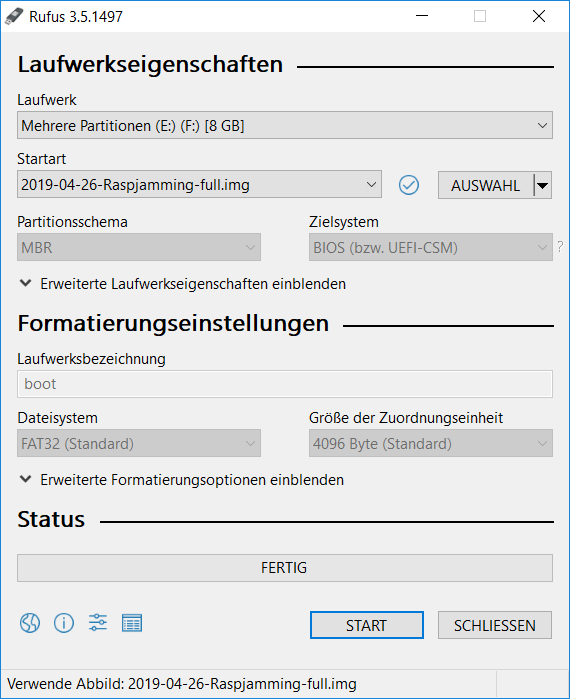
\includegraphics[scale=0.5]{images/Rufus_Raspjamming.png}
	\label{Rufus}
\end{figure}

Nun kann die MicroSD-Karte in den Raspberry Pi gesteckt und an die Versorgung angeschlossen werden.

